\chapter{The Mendelian Basis of Inheritance}
\label{cha:mendelian-basis-of-inheritance}

\section*{PARTICULATE AND DUPLICATE NATURE OF INHERITANCE}

The essence of Mendelism is that inheritance is by particles or units
(called genes hereafter) and that these genes are present in pairs, one
member of each pair having come from each parent. Each gene maintains
its identity generation after generation instead of blending with
the other genes to form a new kind or blend of
\index{``Blending inheritance''}hereditary substance, as
was thought in pre-Mendelian days. When the individual reproduces,
it transmits to each offspring one or the other, but not both, of the
genes in each pair it possesses. thus the parent gives to each offspring
\textit{only a sample half of its own inheritance}. The laws of chance govern
this sampling, subject to the restriction that each sample must contain
one gene of every pair. This sampling nature of the process of inheritance,
scarcely suspected in pre-Mendelian days, allows a parent to transmit
different inheritance to different offspring. More precisely, if we
let \textit{Aa} represent a pair of genes in a parent which has two offspring,
there is one chance in four (the exact result in individual cases varying,
of course, according to the laws of sampling) that both offspring will
get \textit{A}. There is one chance in four that both will get \textit{a} and there are two
chances in four that one will get \textit{A} and the other will get \textit{a}. Similar
probabilities apply to every other pair of genes. Thus, about half of the
genes which two offspring receive from the same parent (i.e., about
one-fourth of all the genes they have) are exact duplicates; but the
other genes the two get from that parent (another fourth of all the
genes they have) were opposite members of the pairs in that parent. In
those pairs of genes for which the parent was homozygous it will not
matter which gene of the pair is transmitted, for the result will be the
same with either. Most parents are heterozygous for many pairs of
genes. Here lies the explanation of the fact that identical pedigrees do
not mean identical inheritance, although they usually do mean a considerable
degree of likeness.\footnote{To illustrate the Mendelian basis for the fact
that identity of pedigree generally means similarity but not identity of
inheritance, let us consider the probable results of a particular mating in
a breed heterozygous for many pairs of genes and mating at random with
respect to each pair. If the contrasting alleles in each pair are equally
frequent in the breed, then the most probable Mendelian formula of mates
chosen at random can be illustrated as below, the mates being alike in some genes
and unlike in others. How many different kinds of full sibs could there be from this
particular mating? How many different kinds of half sibs could come from this one sire
(or dam) mated to all the different kinds of mates which exist in the breed? How many
different kinds of individuals can exist in the entire breed? The Mendelian formulae
of the parents and the answers to each of these three questions may be indicated as
follows:

Formula of sire: \textit{AABbccDdeeFfGGHhli]jKKIIMMNnooPp}

Formula of dam: \textit{AABbCcDDeeffGgHhii]jKkLLmmNNOoPp}

Kinds of full sibs: lx3x2x2xlx2x2x3x2x3x2xlxlx2x2x3 = 20,736

Kinds of paternal half sibs: 2x3x2x3x2x3x2x3x3x3x2x2x2x3x2x3 = 1,679,616

Kinds in breed: 3x3x3x3x3x3x3x3x3x3x3x3x3x3x3x3 = 43,046,721

Since there are more than twenty thousand kinds of full sibs possible from this
mating, it is unlikely that two full sibs even from among a large number would happen
to be exactly alike. Yet less than one two-thousandth of the total number of kinds
of individuals possible in the whole breed are possible at all in this particular set of
full sibs. This sire could not possibly sire a twenty-fifth of the kinds possible in the
whole breed, no matter what kind of mates he had. This example is schematic in two
important respects: first, many more than 16 pairs of genes are doubtless heterozygous
in all breeds; and, second, it would be a surprising coincidence if the unlike
alleles were equally numerous in more than a few of those pairs.} That identity of pedigree
(as of full brothers) does not mean identical heredity was well known in pre-Mendelian
days but either was regarded as one of the unexplained mysteries of
heredity or interpreted to mean that a large amount of entirely new
inheritance (mutations we would say today) had arisen in each individual.
\index{Genes, nature of}

\index{Sampling nature of inheritance|(}
Since half of the inheritance comes from each parent, except in the
case of sex-linked genes, and since in each pair the gene received from
the sire and gene received from the dam are equally likely to be transmitted
to any one offspring, most of the facts of inheritance when
expressed in quantitative form involve the fraction l/2. It is only a
small exaggeration to say that the mathematics of genetics is the algebra
of 1/2!

\index{Allele}\index{Dominance}Dominance is not an essential part of Mendelism, although Mendel
himself noted it. It is a ready explanation of some cases of ``reversion''
or \index{Atavism}``atavism,'' but not the only explanation for those. The chief part
played by dominance is to increase the variability of the population
slightly and to make certain genotypes indistinguishable from each
other. There is nothing in the mechanism of inheritance which would
cause a dominant gene to increase in numbers at the expense of its
recessive allel, or the reverse. \index{Gene frequency}If \textit{q} is the proportion of \textit{A} genes and
$1 - q$ is the proportion of \textit{a} genes in the population and \textit{p} is the
proportion of heterozygotes, then no matter what system of mating prevails,
the zygotic ratio\index{Zygotic ratios} will be $(q - p/2)AA:p Aa: (1 - q - p/2) aa$.
If these have equal opportunity to reproduce (that is, if no selection for
or against either of the three genotypes prevails), then the proportion
of \textit{A} genes in the next generation will be $q - p/2$ from the \textit{AA individuals
plus} $p/2$ from the \textit{Aa} individuals which equals \textit{q} in the whole
population, the same as it was in the preceding generation. Without
selection the Mendelian mechanism itself does not change gene ratios
except, of course, that it permits sampling variations to occur in the
segregation process at each generation. Those are slight except in very
small populations. There they cause the phenomena of inbreeding.
\index{Sampling nature of inheritance|)}

\section*{POST-MENDELIAN ADDITIONS TO THE LAWS OF INHERITANCE}
\index{Linkage|(}

Mendel knew nothing of \index{Chromosomes|(}\textit{chromosomes} or \textit{linkage}. The achievements
of genetics in the last third of a century in identifying the
chromosomes as the carriers of the genes have not changed the laws
which Mendel discovered, except to modify the law of independent
assortment so that it is now known to apply only to genes which are on
different chromosomes. Cytological investigations of the mammals and
birds are unusually difficult because the number of chromosome pairs
is large, the chromosomes are small, and the processes of killing, fixing,
and staining are apt to cause the chromosomes to ``clump'' together, so
that the observer cannot be sure how many there are.

Because of these difficulties, mammalian and avian chromosomes
have not been so well investigated as those of most farm crops and of
many lower animals. In several cases investigators do not yet agree in
their counts. Some species have been studied by only one investigator.
Most of the findings quoted in table~\ref{tbl:Lush_Table_1} are still subject to confirmation.\footnote{For a
more complete list and references, see: Oguma, Kan, and Kakino, Sajiro.
1932. A revised check-list of the chromosome number in vertebrata. \textit{Jour. of Genetics},
26:239--54, and for birds: Miller, R. A. 1938. \textit{Anatomical Record} 70:156--58.}
Work much older than 1920 is quoted only where no subsequent work
has been reported, or where this earlier work has been quoted widely.
In general the later work is more apt to be correct. On account of the
``clumping,'' the larger numbers are more likely to be correct wherever
there is not yet substantial agreement.

Most farm animals have around 20 to 30 pairs of chromosomes;
hence two genes chosen at random will nearly always be independent of
each other. Yet if one is considering a trait affected by more than six or
seven pairs of genes, there is likely to be linkage among some of them.\footnote{The
chicken, the mouse, and the rat are the only farm animals for which the
construction of linkage maps is yet well along. See \textit{Jour. of Heredity} 3l:232--35 and
36:271--73. Some mapping has begun with the silkworm and with cattle.}
On account of linkage, genes which were transmitted to the parent
together (i.e., which both came to it from the same one of its parents)
will be transmitted together to the offspring more often than if they
were independent. Yet in the population as. a whole, if crossing-over
occurs at all, \index{Coupling and repulsion} the ``repulsion'' and ``coupling'' phases soon become equally
frequent, thus causing linkage to hinder selection (in a hitherto
unselected population) in about as many cases as it helps. Hence linkage
does not offer the breeder much chance to get one gene by selecting
another closely linked to it. The effects of linkage in causing two genes
or characteristics to be together or apart more often than not are conspicuous
only in the first few generations after a cross between two
unusually homozygous races-a condition which rarely confronts the
animal breeder under our present purebreeding systems. The existence
of linkage causes the genes to tend to segregate in large groups at any
one cell division and hence causes the population to behave as if there
were fewer genes than there actually are. But this effect is probably
unimportant, since the cross-overs in different cells, even in the same
individual, may be at various places on the chromosomes and since
genes with opposite effects are as likely to be linked together as are
genes with similar effects. Linkage is some hindrance to progress by
selection (after the first generation) since it keeps desired and undesired
genes from recombining into separate gametes as often as they
would if not linked. This lessens slightly the variability among the
immediate offspring of selected parents and consequently reduces the
amount which can be accomplished by selecting among them.

\begin{small}
	\label{tbl:Lush_Table_1}
	\setlength\LTcapwidth{\textwidth} % default: 4in (rather less than \textwidth...)
	\setlength\LTleft{0pt}            % default: \parindent
	\setlength\LTright{0pt}           % default: \fill
	\begin{longtable}{@{\extracolsep{\fill}}b{2cm}|b{2cm}|b{2cm}|b{4cm}}
		\caption{\textsc{Recent Reports of Chromosome Numbers in Mammals and Poultry}}\\
		\hline
		\hline
		Animal 				& Number of Pairs of Chromosomes & Heterogametic Sex & Investigator and Date of Publication \\
		\hline
		\endfirsthead
		\caption[]{\textit{Continued}}\\
		\hline
		\hline
		Animal 				& Number of Pairs of Chromosomes & Heterogametic Sex & Investigator and Date of Publication \\
		\hline
		\endhead
		Farm animals: 		&                     	&        			& \\
		\tabindent Horse    & 30                  	& Male   			& Painter, 1945 \\
		              		& 19                  	& Male   			& Wodsedalek, 1914 \\
		              		& 19                  	& Male   			& Masui, 1919 \\
		\tabindent Ass      & 32                  	& \ldots 			& Sokolov, 1937 \\
		\tabindent Mule     & Unpaired, 51 in all 	& \ldots 			& Wodsedalek, 1916 \\
		\tabindent Camel    & 35                  	& \ldots 			& Novikov, 1940 \\
		\tabindent Cattle   & 30                  	& Male   			& Krallinger, 1930 \\
	    	          		& 19                  	& Male   			& Wodsedalek, 1920 \\
	        	      		& 30                  	& Male   			& Makino, 1944 \\
		\tabindent Yak		& 30					& \ldots 			& Zuitin, 1938 \\
		\tabindent Buffalo	& 30					& \ldots			& Pchakadse, 1939 \\
							& 24					& \ldots			& Makino, 1944 \\
		\tabindent Sheep	& 27					& Male				& Berry, 1941 \\
							& 30					& Male				& Several workers, 1931 to 1940 \\
		\tabindent Goat		& 30					& Male				& Krallinger, 1931 \\
							& 30					& Male				& Warwick, 1935 \\
		\tabindent Swine	& 19					& Male				& Krallinger, 1936 \\
							& 19					& Male				& Crew and Koller, 1939 \\
		\tabindent Dog		& 26 $\pm$				& Male				& Painter, 1925 \\
							& 39					& Male				& Ahmed, 1941 \\
		\tabindent Cat		& 19					& Male				& Minouchi, 1928 \\
							& 19					& Male				& Koller, 1941 \\
		Farm poultry:		&						&					& \\
		\tabindent Chicken	& 33					& Female			& White, 1932 \\
		\hline		
		\tabindent Chicken	& 39					& Female			& Yamashima, 1944 \\
							& 40					& Female			& Miller, 1938 \\
							& 16 to 37				& Female			& Various authors since 1923 \\
		\tabindent Duck		& 38 to 39				& Female			& Werner, 1927 \\
							& 39					& Female			& Sokolov, \textit{et al.}, 1936 \\
		\tabindent Turkey	& 23 to 29				& Female			& Various authors 1929 to 1936 \\
		\tabindent Peacock	& 18 to 29				& Female			& Tiniakow, 1934 \\
		\tabindent Pigeon	& 31					& Female			& Oguma, 1927 \\
							& 25 $\pm$				& Female			& Hance, 1933 \\
							& 24 $\pm$				& Female			& Painter and Cole, 1943 \\
		Various mammals:	&						&					& \\
		\tabindent Man		& 24					& Male				& Many recent authors \\
		\tabindent Chimpanzee			& 24					& Male ?			& Yeager \textit{et al.}, 1940 \\
		\tabindent Old World monkey	& 27					& Male				& Painter, 1925 \\
		\tabindent New World monkey	& 27					& Male				& Painter, 1925 \\
		\tabindent Nyctereutes (raccoon dog)	& 21			& Male				& Minouchi, 1929 \\
		\tabindent Red fox				& 21					& Male				& Wodsedalek, 1931 \\
		\tabindent Fox:		&						&					& \\
		\hspace{6mm} V. vulpes			& 17					& \ldots			& Andres, 1938 and Wipf, 1942 \\
		\hspace{6mm} V. lagopus			& 26					& \ldots			& Andres, 1938 \\
		\hspace{6mm} V. fulva			& 16					& Male				& Bishop, 1942 \\
		\tabindent Rat		& 21					& Male				& Many recent authors \\
		\tabindent Mouse	& 20					& Male				& Many recent authors \\
		\tabindent Deer mice (Peromyscus) &	24 to 29		& \ldots			& Cross, 1938 \\
		\tabindent Rabbit	& 22					& Male				& Painter, 1926 \\
		\tabindent Rabbit	& 22					& Male				& Minouchi and Ohta, 1932 \\
		\tabindent Guinea pig			& 19					& Male				& Harman and Root, 1926 \\
							& 31					& Male				& League, 1928 \\
							& 33					& Male				& Mols, 1928 \\
		\tabindent Mink		& 14					& Male				& Schackelford and Wipf, 1947 \\
		\tabindent Hamster, golden		& 19					& Male				& Koller, 1938 \\
		\hline
		\tabindent Hamster, striped	& 7						& Male				& Pontecorvo, 1943 \\
		\tabindent Twelve other species of rodents	& 22 to 43 (only 3 above 27)	& \ldots	& Cross, 1931 \\
		\tabindent Peccary	& 15					& \ldots			& Krallinger, 1936 \\
		\tabindent Armadillo			& 30					& \ldots			& Painter, 1925 \\
		\tabindent Bat		& 24					& Male ?			& Painter, 1925 \\
		\tabindent Hedgehog	& 24					& \ldots			& Painter, 1925 \\
		\tabindent Opossum	& 11					& Male				& Hoy and George, 1929 \\
						& 11					& Male				& Painter, 1925 \\
		\tabindent Kangaroo	& 6						& \ldots			& Painter, 1925 \\
		\tabindent Eight other genera of marsupials	& 6 to 10	& Male	& Various authors \\
		\hline
	\end{longtable}
\end{small}

Mendel did not know of sex-linkage\index{Sex linkage} which, in the heterogametic sex, is an exception to the rule that
inheritance is in duplicate and comes equally from both parents. Only one pair of chromosomes carries
the sex-linked genes. Presumably something like one-twentieth or one-thirtieth of all the genes are
sex-linked, although that is only a rough approximation since the sex-chromosomes might carry more or
less than their proportionate share of the genes. To ignore sex-linkage will generally lead to but
little error; yet there doubtless is some sex-linkage in all farm animals, and probably there are
occasional characteristics which are affected by a disproportionately large share of sex-linked
genes. The general effect of sex-linkage is to make parent and offspring of opposite sex resemble
each other slightly more than parent and offspring of the same sex do. Here and there it has some
conspicuous special effect, such as making possible, in some matings, the identification of sex in
very young poultry. Partial sex-linkage is known genetically in man and presumably exists in all other
mammals in which portions of the X-chromosome cross over with portions of the Y-chromosome. The
practical consequences are like those of sex-linkage but even less noticeable.
\index{Chromosomes|)}
\index{Linkage|)}

\section*{IS THERE ANY NON-MENDELIAN INHERITANCE}
\index{Non-Mendelian inheritance|(}
\index{Polyploidy|(}

Each year of genetic research brings added evidence that all inheritance is Mendelian in the broad
sense of being in duplicate and particulate, with the particles maintaining their identity. The only
well-established exceptions are plastid inheritance, known only from plants, and polyploidy, where
inheritance is particulate but present in more than duplicate. Polyploidy seems to be very rare in
animals, although it appears to have been important in the evolutionary history of the plant kingdom.
On account of the sampling nature of inheritance, polyploidy must be a temporary condition lasting only
a few generations until the polyploid individuals either die out or develop a new diploid division
among their chromosomes. A few cases of inheritance through the maternal line only have been reported.
Most of those have later been found to require some other explanation. Often it is found by further
experiment that these were characteristics for which the unfertilized ovum was already organized and the
genes which the sperm brought are merely delayed a generation in expressing their effects. Whether the
shells of certain snails coil to the left or to the right is an example.

It may never be possible to prove rigorously that all inheritance is Mendelian in this sense, for so long
as the inheritance of any characteristic is unknown, an obstinate skeptic might still say: ``Perhaps the
inheritance of that characteristic conforms to some other rule.'' It is a fact, however, that many cases
of inheritance which were at one time thought not to behave in the Mendelian manner, have been shown by
more thorough analysis to behave in that very way except that the number of factors is large or that the
interactions between different factors are unusually complicated or that the egg was already so highly
organized that the genes in the sperm cell could not show some of their effects until the next generation.
Moreover, the ineffectiveness of selection within pure lines seems to be some positive evidence that there
can be no appreciable amount of truly ``blending'' inheritance. (Cf. Fisher, pp. 17--18.)
\index{Non-Mendelian inheritance|)}
\index{Polyploidy|)}

\section*{THE NUMBER OF GENES}
\index{Genes, number of|(}

There are at least four kinds of evidence which show something about the total number of pairs of genes in
certain species. They leave little doubt that the breeder of farm animals must contend with a genetic
situation in which the number of different pairs of genes heterozygous in his herd or flock is at least
many scores, probably many hundreds, and perhaps even a few thousands.

The first kind of evidence is the number of genes which have actually been found in the organisms studied
most. In \textit{Drosophila melanogaster} more than 500 different loci have already been located on the
chromosome maps, and many more are known. In \textit{D. pseudoobscura} there are in the third chromosome
alone at least 289 loci which can mutate to lethal genes (\textit{Genetics} 26:39). Baur and his co-workers
found some 300 genes in the snapdragon, \textit{Antirrhinum majus}. In corn (\textit{Zea mays}) some 400
genes had been catalogued up to 1935 (Rhoades and McClintock). In the wasp, \textit{Habrobracon juglandis},
about 100 mutations at separate loci are known. In \textit{Datura} (the genus which includes the Jimsonweed)
about 500 genes were known, 77 of them located on the chromosome map, by 194l. The inherilance of more than
100 characters has been studied in barley (\textit{Genetics} 28:419). In man more than 200 genes have been
reported, some 45 of them on the X-chromosome, but the evidence for many of those is scanty because controlled
experimental matings are not possible. The number of genes reported for most species of farm animals is only\
a few dozen,\footnote{For example, Ibsen in 1933 listed 17 pairs of genes and one multiple allelic series of
genes affecting color in cattle. He mentions several other color characteristics, the mode of inheritance of
which was not yet clarified. In the fowl 21 genes are already (1940) located in six linkage groups
(\textit{Jour. of Heredity} 31:231--35), and other genes are known but not located.} and many of those are not
very certainly established, but only a few thousand farm animals have been observed under such circumstances
that genes would have been identified readily.

This kind of evidence has two limitations: First, only genes with effects conspicuous enough to permit their
ready identification can be catalogued in the Mendelian manner. Genes with minor effects can only be lumped
together in an indefinite background of ``modifying factors.'' Second, the number already found provides
scarcely any basis for guessing whether that number is only a tiny fraction or a large fraction of the total
number which exists. Certainly the number reported is less than the actual number.

A second kind of evidence comes from cytology. Work (\textit{Journal of Heredity} 33:403--7, 1942.) on the
\index{Chromosomes}chromosomes in the salivary glands of Drosophila shows about 5,000 distinct bands; and the cytogenetics of
deletions, inversions, etc., makes it seem plausible that each of these is a gene, although it remains
possible that there may be several genes in some bands. Belling in studying the chromosomes of the lily was
able to distinguish about 2,200 to 2,500 ``chromomeres,'' or distinct segments of its chromosomes; but the
genetics of the lily is not well enough known to show how closely the genes and the chromomeres correspond
to each other. Each chromosome in the farm animals surely must carry many genes; but the cytology of mammals
and birds is difficult and little except number is known of it so far.

A third kind of evidence comes from some indirect reasoning, based on the number of times certain mutations\index{Mutations}
recurred. The first such estimate was a figure of about l,800 loci, but it was recognized that the
assumptions involved made this lower than the true figure. Gowen and Gay in 1933 reached an estimate of
14,280 loci in Drosophila. This estimate had a large sampling error but was thought to have no consistent
bias either in the direction of largeness or of smallness. Muller and Prokofyeva in 1935 reached the
conclusion that in Drosophila the total number of loci ``\ldots is of the order of a few (ca. 5--10)
thousand.''

A fourth kind of evidence comes from the experiments on quantitative inheritance\index{Quantitative inheritance} which require for their
interpretation a minimum number of genes if those express their effects in the very simplest way (i.e.,
without dominance or other nonadditive interactions). Sumner's experiments with mice of the genus Peromyscus
showed that many of the quantitative characteristics in which two varieties or local races differed were
each affected by many genes for which neither population was homozygous. ``Student'' interpreted the Illinois
Agricultural Experiment Station's work in selecting corn for high and for low oil content as showing that the
oil percentage in the initial stock of corn ``\ldots was conditioned by the presence, or absence, of a number
of genes, at least of the order 20-40, possibly of 200-400, and not at all likely to be of the order 5-10.''\index{Selection}
The Illinois Station's work with the Bowlker herd, which was produced by crossing Guernseys and Holstein-
Friesians, has been interpreted (page 123, Annual Report for 1928--29) as requiring more than 10 pairs of
genes to explain the \index{Breed differences}breed difference in milk yield and several more pairs of genes to explain the breed
difference in the percentage of fat. The Tranekjaer experiments with Jersey and Red Danish cattle in Denmark
indicate that at least seven pairs of genes were concerned with the difference in fat percentage between those
breeds.\footnote{Wriedt postulated that one pair of genes would account for the breed difference; but, as
Skovsted pointed out, not enough of the parental types reappeared in the back-crosses or in the $F_2$ to justify
that. The figure seven mentioned here is based on comparisons of parental means and $F_1$ , $F_2$, and back-
cross variabilities.} Jull concludes that in the fowl sexual maturity, rate of laying, and persistency of laying
are each ``\ldots affected by a relatively large number of genes, some of which probably influence more than one
character.'' Many other examples might be cited, each yielding figures of from 4 or 5 up to more than 20 as the
minimum number of pairs of genes affecting a given quantitative characteristic.

The usual result of an experiment on the genetics of a quantitative
characteristic is that the number of genes involved ``cannot be less
than'' a certain number, but might be larger. Usually the longer the
genetic investigation continues, the more genes are found. In such
experiments the evidence which throws light on gene number usually
involves differences between the parental means and between the variabilities
of the parental groups, the $F_1$ or the $F_2$ or the back-crosses, or it
concerns the change produced in the mean and in the variability by a
given amount of selection. Often the numbers are small and the sampling
errors are high. Those may make the answer obtained either too
large or too small. Nearly all other sources of error make the answer
smaller than it should be. Thus, this kind of evidence can only show
that the number of genes is more than a certain small number which,
however, is usually too large to leave any reasonable hope that even the
most thorough study will enable a breeder to know the Mendelian
formula for all the important genes in any of his animals.

\index{Genes, nature of|(}
A fifth line of reasoning, which perhaps scarcely deserves to be called
evidence until more is known about the physiology of how the genes
produce their effects,\footnote{See \textit{Quart. Rev. of Biology}
13:140--68 and \textit{Physiological Reviews} 21:487--527.} is that the
development and functioning of each
organ in the animal is so complex and is dependent upon such a delicate
interplay of various tissues, hormones, fluids, etc., each acting at
the proper time, that it is scarcely conceivable that a small number of
genes can initiate and control all of this. The term ``unit character''\index{Unit character}
which was freely used in the early days of genetics tends to be avoided
now, lest it confuse by implying that one gene by itself is enough to produce
the whole characteristic. The gene, not the characteristic, is the
unit of Mendelism. In a sense it may be legitimate (and it is often convenient)
to refer to \textit{the contrast} between two characteristics --- for example,
red eye and white eye in Drosophila --- as a unit character since, in
some matings at least, the difference between the two characteristics is
caused by a difference in only one pair of genes. Yet it is confusing to
speak of \textit{red eye} as a unit character, since more than 40 genes have been
found thus far which must all be present if the usual red eye of the wild
fly is to develop. If one of them is absent, the eye may be ``purple''`; if
another is absent, it may be ``peach''; etc.; but the co-operation of them
all (and doubtless of still unknown genes) is required to produce the
normal eye. The cooperation of at least 100 genes is necessary to
produce normal green chlorophyll color in corn. (\textit{Amer. Nat.} 80:431).

The fact that many distinct abnormalities and defects are caused by
a change in only one gene is to be expected if that gene interrupts, at
some important stage for which there is no substitute, the long chain of
physiologic processes by which the normal characteristic usually develops.
For example, in the normal process of horn formation in cattle
there may be several stages which, if interrupted, would alter or prevent
all the later stages of development; but it is not easy to imagine that
any one gene could guide the whole course of horn development,
including the growth of the bony core, the blood vessels, nerves, etc.
Thus, it may be legitimate to speak of a single gene for hornlessness:
but it is not legitimate to infer that the allelic gene to that one is the
gene which produces horns. The case is analogous to that of destroying
a house by a single act, such as applying a match to it at any one of a
number of places. But a house can be built only by the timely co-operation
of an enormous number of individual acts. It is scarcely legitimate
to speak of refraining from applying the match as an act which builds
the house.

The eradication of single-gene defects, such as lethals and semilethals,
may be an important part of the task of animal breeding; but its
practical importance can scarcely approach that of changing the fertility,
vitality, growth rates, proportions of conformation, milk production,
speed, wool production, etc., which are most of the economic
differences between ordinary or moderately inferior and distinctly
superior animals. The genetic evidence indicates that these are complex
physiological characteristics i zn which most of the hereditary
differences are caused by a large number of genes, each with an individually
small effect.
\index{Genes, nature of|)}

\section*{CONSEQUENCES OF THE LARGE NUMBER OF GENES}
\index{Gametic ratio}
\index{Variation!as affected by gene numbers|(}

When only one pair of genes is concerned, two kinds of gametes and
three kinds of genotypes are possible. If there are two pairs of genes,
each possibility for the one may occur in combination with each possibility
of the other, thus permitting four kinds of gametes and nine
kinds of genotypes. Three pairs of genes permit 8 kinds of gametes and
27 kinds of genotypes. The general formulae are: the number of kinds
of gametes or of homozygous genotypes possible with n pairs of genes is
$2^n$ (which may be written $10^{.301n}$; the number of different kinds of
genotypes possible is $3^n$ (which may be writen $10^{.477n}$). These numbers
become big beyond human comprehension if \textit{n} is very large. Even if
there are only 100 pairs of genes, 31 digits will be needed for writing
the number of kinds of gametes possible; and there will be 48 digits in
the number of kinds of genotypes possible. The possibilities for hereditary
differences under this system are enormous. They may be visualized
by comparing them with the number of animals of each species
actually alive in the whole world at any one time. During the years
around 1926 to 1935 these were as follows for man and for some of the
more important farm animals (figures from USDA Yearbooks):

\begin{table}[htbp]
	\centering
	\begin{tabular}{lr}
 						& \textsc{Tens of Millions} \\
		Human beings	& 200 \\
		Cattle			& 70 \\
		Horses			& 10 \\
		Mules and asses	& 3 \\
		Sheep			& 69 to 74 \\
		Swine			& 25 to 28 \\
		Chickens (in the United States only)	& 44 \\
	\end{tabular}
\end{table}

Hence, if the number of different genes heterozygous in each species
is as large as 40 (and it may well be thousands), the number of different
hereditary combinations possible in each species is millions on millions
of times as large as the number of animals which can actually be alive
at any one time. It would be a remarkable coincidence if any two living
things were exactly alike in all their heredity, except for a few special
cases such as identical twins, asexually reproduced organisms, and possibly
members of a strain which had been very highly inbred for a long
time. Gesell says (\textit{Science} 88:227): ``Even in the detailed studies of animal
respiration, it has been found that no two dogs breathe exactly
alike.''

\index{Multiple alleles|(}
Another comparison to show vividly the enormous number of different
kinds of individuals possible is furnished by the physicists' estimate
that the number of electrons in the universe is about $10^{80}$. In a
species in which only 200 pairs of genes are heterozygous there could be
$10^{95}$ different kinds of individuals. This is a million billion times as
many as there are electrons in the universe!

In these calculations it was assumed that there are only two allelic
genes in each series. In several cases it is already known that there are
three or more different kinds of genes in an allelic series (called ``multiple
alleles'' in genetics), and it is possible that all allelic series are potentially
multiple.\footnote{Several series have already been found in which there are more than four
alleles. The albino series in the rabbit is an example. The maximum numher yet
reported in any organism is 45 alleles for a self-sterility gene in one of the primroses,
\textit{Oenothera organensis}. \textit{Genetics} 26:469. More than 22 alleles are known in the white
eye series in \textit{Drosophila melanogaster} and more than 40 at the locus for ``bobbed.''
In man at least four alleles exist to determine the blood types. $A$, $A^1$, $B$, and $0$, and
more than a half dozen alleles at the locus for the \textit{rh} blood factor have been reported.}
This increases the number of kinds of gametes and
genotypes possible. If \textit{m} alleles are possible in each of \textit{n} allelic series,
the number of different kinds of gametes possible is $m^n$ and the number
of different kinds of genotypes possible is $ \left[ \frac{m(m+1)}{2} \right]^2 $.

Linkage\index{Linkage|(} does not affect the number of kinds of gametes which may
be produced but does affect their proportions and thereby increases the
size of population necessary to permit all kinds of genotypes to be produced.
Also, it increases the number of genotypes possible because the
multiple heterozygotes will now be different genotypes according to
whether the linkage is in the coupling or repulsion phase. That is, $\frac{AB}{ab}$
and $\frac{Ab}{aB}$ will be different genotypes if linkage exists, whereas both
would have been the same genotype, \textit{AaBb}, if there had been no linkage.
A triple heterozygote, where all three genes are linked, can exist
in four different genotypes, a quadruple heterozygote in eight genotypes,
etc.

Both these additional complications --- multiple alleles and linkage --- increase
the number of kinds of genotypes possible. Unless the number
of heterozygous genes is very small, there is no escaping the conclusion
that the number of genetically different kinds of individuals possible in
a breed or species is practically infinite. Except in the rare case of identical
twins, one can confidently expect to breed cattle, or any other
species of farm animal, a lifetime without ever having a second animal
exactly like one he produced earlier.

If each gene had a different kind of effect and there was no confusion
by environmentally caused variations or by \index{Dominance}dominance, the number
of kinds of animals different in appearance or performance would
be the same as the number of kinds of genotypes. If all pairs of genes
showed complete dominance, but each pair of genes had a different
effect, the number of kinds of animals would be the same as the number
of kinds of gametes. But if very many genes are involved, some will
produce effects like those of others, some will produce effects only when
certain others are present, and some will produce the same effects as
variations in environment do. Therefore, if the genetic situation is at
all complicated, the outwardly distinguishable kinds of animals grade
into each other in an almost continuous series. When we classify a large
group of animals on the basis of outward appearance or performance
in any one characteristic, even with considerable precision, we are
almost certain to include in each class many genetically different kinds
of individuals.
\index{Genes, number of|)}
\index{Linkage|)}
\index{Multiple alleles|)}
\index{Variation!as affected by gene numbers|)}

\section*{THE GENETIC INTERPRETATION OF THE ``PURITY'' OF PURE BREEDS}
\index{Breed purity|(}
\index{Heterozygosis|(}
\index{Homozygosis|(}

In animal breeding usage, purity of breeding refers to ancestry and
is not the same as the genetic term ``homozygosity,'' although there is
some slight relationship between the two. The purebred animal is one
whose ancestors all belonged to that same breed for as far back as is
required by the rules governing registration in that breed. Since all
breeds are finitely limited in the number of animals alive at any one
time, and many breeds were very small in numbers for a long time during
their formative period, a certain amount of homozygosity was produced
by the resultant inbreeding\index{Inbreeding|(}. This is usually a faint force in
pure breeding as practiced today in breeds which have become large and
successful, but occasionally was intense during the formative period
when the breed was very small. The Shorthorn breed, which has the
oldest pedigree record, probably lost through the inbreeding process
about 25 or 30 per cent of its initial heterozygosity in the century and a
third from its foundation to 1920. Most of this was lost in the formative
stage while the ancestry of the future breed was largely included in the
herds of the Colling brothers, who both shaped their breeding operations
to an unusual degree around one bull, Favourite. In most breeds
yet studied, the breed is now losing something like one-half of one per
cent of its heterozygosis per generation. In breeds of cattle and sheep,
where the average length of generation is around four or five years, this
would mean that in a century the mere fact of absolute purity of breeding
would cause a decrease of about 10 per cent in the amount of heterozygosity
initially present. This would be partially offset by the
occasional registration of a grade through fraud, accident, or official
permission, and by the new mutations which might occur and survive
during that century. In addition to these three processes of inbreeding,
introduction of outside blood, and mutation\index{Mutations|(}, selection may have helped
either to increase or to decrease the average homozygosity of the breed.
Selection, however --- in marked contrast to its effectiveness in changing
average merit --- is a very feeble tool for changing homozygosity, except
under the very simplest genetic situations, as we shall see in chapter 11.
It is not likely, therefore, that selection has made much change in the
average homozygosity of the pure breeds since they were first separated
from the general population, although it has certainly changed the
breed averages distinctly in many cases.

\index{Selection}
It is sometimes argued that, while the total number of genes may
perhaps run into the thousands, yet most breeds (or subgroups of a
species in nature) will be homozygous for all but a few of those. This
seems improbable, since no genetic mechanism is known by which that
condition would be likely to be attained in the first place nor by which
it could be maintained very long if it ever were reached. If a breed or
species ever became entirely homozygous for a given pair of genes,
mutations --- even at a very low rate --- would cause that homozygosis to be
lost bit by bit. Selection is too feeble to restore complete homozygosity
as rapidly as mutation destroys it, especially if the mutations are usually
recessive, although selection is amply powerful to keep consistently
undesirable mutant genes from becoming abundant. Inbreeding can be
powerful enough to restore that homozygosity, but it is doubtful whether
it often is intense enough in nature or in the breeding of large and
popular breeds to achieve that end. Wright estimates\footnote{\textit{Genetics},
16:119--21. See also table 5 in Fisher's
\textit{Genetical Theory of Natural Selection}.} that a freely
interbreeding species of one million individuals at equilibrium with
one new mutation in each 1,000 individuals could support permanently
some 30,000 unfixed loci, which is larger than any of the current estimates
of total gene number. In other words, few genes in such a species
would be entirely homozygous all through the species. Smaller species
would not support so many\footnote{The same formula gives nearly 2,560 as
the number of unfixed loci in a species of 100,000 individuals, 210 in a species
of 10,000 and 16 in a species of only 1,000. Our ignorance of whether the rate
postulated for mutation is too high or too low and our ignorance of whether the
effective number of breeding individuals is far smaller or only a little smaller
than the census number prevent us from using these figures with much confidence.}
unfixed loci. The inbreeding which the pure breeds of livestock undergo comes
mostly not from the smallness of the breed in absolute numbers but from the
circumstance that many breeders are simultaneously using sons or grandsons of a
few currently famous sires.\footnote{See Calder's study of the Clydesdale breed
of horses. \textit{Proc. Roy. Soc. Edinburgh} 47 Part 2, No. 8:118--40. 1927.}
When the pure breeds finally reach equilibrium between the production of
heterozygosis by mutations and the loss of heterozygosis because the effective
number of animals in the breed is small, it is possible that the pure breed may
support only a few scores of unfixed loci. But it is unlikely that the pure
breeds have come at all close to that equilibrium point in the comparatively
short time (in terms of animal generations) since they were organized. It seems
entirely conservative to estimate that the average pure breed is still heterozygous
for hundreds of pairs of genes, although, of course, no animal in it is
heterozygous for even half of them and probably no one gene is heterozygous
in even half of the members of a breed.
\index{Breed purity|)}
\index{Heterozygosis|)}
\index{Homozygosis|)}
\index{Inbreeding|)}

\section*{MUTATIONS}

Mutation is a rare process. The mutation rates observed in the laboratory
under otherwise natural conditions are generally around the
magnitude of one mutation of each gene in 100,000 or 1,000,000 generations
(Stadler, Gowen). The rate is not the same for all genes, however,
and can be increased by such extreme environments as exposure to
X-rays, radium, ultraviolet light or barely sublethal temperatures. Also
a few genes which alter the mutation rates of other genes have been
found. Dr. H. D. King observed among 45,000 Norway rats 6 different
mutations affecting hair; but the number of genes affecting hair (i.e.,
the number exposed to mutation) is not known, nor can one be sure
how many mutations with small effects occurred but were not observed.
White and Ibsen estimate (\textit{Jour. Genetics} 32:47) that in cattle the
mutation rate from horned to polled is about one in 20,000. Haldane
estimates that the mutation rate to hemophilia in man is about one in
30,000. More typical is the finding of Dobzhansky and Wright (\textit{Genetics}
26:32) that in the third chromosome of \textit{Drosophila pseudoobscura}
the mutation rate to lethals\index{Lethal genes} must be less than three in 289,000.

If there are 5,000 genes in each individual, then only about one
animal in every 20 or 200 would have even one gene which was a new
mutation. If the breeder were looking for a mutation in one certain
gene, he could expect to find it in only one animal among something
like 100,000 to 1,000,000 animals examined.\footnote{When Warren Gammon
wished to establish a polled variety of purebred Hereford
cattle. he sent about 1,500 letters to breeders inquiring if they knew of such
animals. From the replies he learned of 14 purebred Herefords which were polled,
but some of these animals may have inherited their polledness from the same original
mutation. We can only guess how many horned cattle had been observed by the men
who reported these 14 polled ones, or how many of the 1,500 men who received these
letters knew of polled cattle but neglected to reply.}
Even then, if this mutation produced only a small change in a characteristic also affected by
environment and by other genes, the breeder looking for it would have
only a small chance of recognizing it when he did see it.

Mutations are not only rare, but they are prevailingly harmful. The
larger the change made by a mutation, the less likely is the mutation to
be beneficial to the animal. The reasons for this hinge around the facts
that mutations seem to be random changes in the genes and that any
living animal is already a reasonably successful and highly complicated
mechanism. Any random change in its machinery has only a small
chance of making it a still more successful mechanism but is very apt
to make it operate less well. The bigger the change, the less likely it is
to improve the operation of the mechanism.\footnote{See Fisher's \textit{The
Genetical Theory of Natural Selection}, pp. 38--41, for more detailed reasoning
on this point and for formulae relating the magnitude of a mutation's effect to
the probability of its being beneficial.}
Hence the breeder does not yet have any reason to think that he can help his
practical operations by increasing mutation rates.

Because mutations are rare and prevailingly harmful, the only significance
they have for the breeder is that a tiny part of his efforts in
selection must be spent in keeping these undesired newly mutated
genes from becoming too numerous in the breed. Mutations do have
great significance in evolution because they provide raw material
which can be used by selection and inbreeding or other breeding systems
to change the existing kinds of organisms. Even if only 1 in 1,000
new mutations were beneficial, geologic time is so long that such rare
beneficial mutations may be important in evolutionary changes. Moreover,
mutation serves an important evolutionary purpose by keeping
(against the efforts of selection) a certain store of currently undesirable
genes available in case the environment should change so as to reverse
the direction of selection. For example, suppose a species well adapted
to a life in a humid climate were by migration or change of climate
forced to become better adapted to arid conditions. If mutation has
kept in the species a few genes which make their possessors poorly adapted
to a humid climate but better adapted to an arid climate, then
when the conditions change, some of the newly desirable genes are
already present. Selection may begin at once to increase their frequency.
If mutation had not kept this store of formerly undesirable genes present,
the species might have had to wait for the very slow process of
mutation to produce them after the changed conditions arose. Waiting
for the mutation might have taken so long that the species would have
become extinct first. This consideration may be important in evolution
but probably is rarely of any importance to the practical animal breeder,
since he is concerned with so much shorter periods of time . Perhaps
it might have some slight bearing on such situations as that which
occurred in the American breeds of swine between 1910 and 1920, when
there was a marked change in ideals and the direction of selection in
many particulars was reversed.
\index{Mutations|)}

\section*{GENE FREQUENCY}
\index{Gene frequency|(}
\index{Random mating|(}

A gene may be much more abundant than its allel or it may be
rarer. Gene frequency will be represented here by the letter \textit{q}, which
can have values between zero and 1.0. It is the fraction of the loci of
that allelic series in the whole population which are occupied by the
gene in question. Two examples may illustrate \textit{q} and its variations.
In a count of the colors reported for the 6,000 parents of 3,000 Shorthorns
chosen at random from the British, Canadian, and American herdbooks, Wright
found that 8.6 per cent were white, 43.8 per cent were roan and 47.6 per cent
were red. Assuming that the roan is the heterozygote between the red and white
(which fits the facts better than any other explanation yet advanced, although
there may be some environmental or developmental overlapping between dark roans
and reds), and letting \textit{q} stand for the frequency of the gene for red,
it is obvious that 47.6 per cent of the genes in this locus are genes for red
in the red animals and that 21.9 per cent of the genes in the population are
genes for red in the roan animals, while another 21.9 per cent of the genes in
the population are genes for white in the roan animals. The final 8.6
per cent of the genes which occupy this locus are genes for white in the
white animals. The frequency, \textit{q}, of the gene for red in the whole
population is, therefore, .476 + .219 = .695; while the frequency of the gene
for white is .219 + .086 = .305. If the population had been mating
truly at random, the proportions of red, roan, and white would have
been the square of the ratio of the two kinds of genes, or: $q^2$ reds :
$2q (1 - q)$ roans : $(1 - q)^2$ whites. The actual count shows a slight
excess of roans and corresponding slight deficits of reds and whites, as
follows:

\begin{table}[htbp]
	\begin{tabular}{lccc}
		\hline
		\hline
 		Color	& Actual Percentage	& Expected Percentage	& Excess of Actual \\
 		\hline
		Red		& 47.6				& 48.3					& -.7 \\
		White	& 43.8				& 42.4					& +1.4 \\
		Roan	& 8.6				& 9.3					& -.7 \\
		\hline
	\end{tabular}
\end{table}

\noindent
The discrepancy, although slight, appears to be significant statistically
and is probably to be explained as a result of the practical breeder's
preference for roan and his having observed long ago that the proportion
of roans was higher from matings of white by red than from any
other type of mating. The chief interest in the above example, aside
from its illustrating what is meant by \textit{q}, is that it shows how slight is
the departure from random mating, even in a simple one-factor case
where there is no dominance to confuse and where ideals are such as to
lead to a rather strong effort toward mating unlikes.

\index{Homozygosis}
Another example of gene frequency may be taken from black breeds
of cattle,\footnote{Wisconsin Agr. Exp. Sta., Bul. 313.} such as
the Holstein-Friesian or Aberdeen-Angus, in which something like
one calf in every 100 to 200 purebreds is born red. The difference
between the black and red, in most cases at least, is a single-factor
one; and dominance is so nearly complete that no one has yet
found how to distinguish the homozygous blacks from the heterozygotes,
(i.e., both \textit{BB} and \textit{Bb} individuals are black but the
\textit{bb} individuals are red). If we let \textit{q} represent the
frequency of the gene for black, we cannot obtain its value simply by
adding the proportion of the homozygotes to half of the proportion of
the heterozygotes, as was done in the Shorthorn example, since we cannot
identify the heterozygotes. By assuming random mating with respect to this
gene (which is reasonable, since all parents are \textit{BB} or \textit{Bb},
which cannot be distinguished, and since not much inbreeding is practiced)
we can, however, get an estimate of \textit{q} if we can get a dependable
count of the proportion of red calves born. That proportion should be $(1 - q)^2$
where \textit{q} is the frequency of the gene for black. If the proportion of red
calves born is 1 in 200, then the frequency of the gene for red is $\sqrt{\frac{1}{200}}$
or about 1 in 14 and that of the gene for black is about 13 in 14. Then
about 1 in 7 or 8 among the calves born black is heterozygous and the
others are homozygous.\footnote{The ratio of homozygous dominants to heterozygotes in
a random breeding population will be $\frac{q}{2(1-q)}$.}
The accuracy of this estimate depends upon the accuracy of the observation that 1 calf
in 200 born is red; and this, for obvious reasons, is not very dependable. If the
proportion of purebred calves born red is about 1 in 100, then \textit{q} is about .9
and about one in five or six of the purebred blacks is heterozygous for red. Also the
heterozygotes will not be uniformly distributed all through the breed but will be more
abundant in those herds where heterozygous sires have been used recently.

Gene frequency will be low for genes against which selection has
already been directed for many generations, as is the case with most
lethals. There is no \textit{a priori} way of estimating whether it will
be high or low for genes which have been the object of selection for only
a few generations or for genes affecting the magnitude of a characteristic
for which the ideal is genetically an intermediate. In populations which
have been very small for a long time or are otherwise intensely inbred,
more genes will be fixed, or nearly so (i.e., they will have values at or
near zero or 1.0); and fewer genes will have frequencies near one-half
than will be the case in large random-bred populations under otherwise
similar circumstances.

In the case of multiple alleles\index{Multiple alleles}, it is usually sufficient to let \textit{q}
represent the frequency of the most desirable gene of the series, grouping
all the other alleles together as less desirable and having a total frequency
of $1 - q$.

\section*{THE BINOMIAL DISTRIBUTION OF ZYGOTES}
\index{Binomial distribution|(}
\index{Gametic ratio|(}
\index{Heterozygosis|(}
\index{Zygotic ratios|(}

If mating is random, the proportions in which the zygotes occur will
be the square of the gametic ratio, as shown in Table~\ref{tbl:Lush_Table_2}.
The typical Mendelian $F_2$ or unselected $F_3$ ratio is merely a special case
of the binomial distribution where \textit{q} happens to be exactly .5. Even small
variations in \textit{q} affect rather strongly the proportions of \textit{AA} and
of \textit{aa}. However, the variations in the proportions of \textit{AA} and
\textit{aa} cancel each other to some extent so that the percentage of heterozygosis
changes only a little with variations in \textit{q}, particularly when \textit{q}
is anywhere near one-half. For instance, it may be seen from Table~\ref{tbl:Lush_Table_2}
and Figure~\ref{fig:Lush_Figure_3} that the percentage of heterozygosis varies only from
.32 to .50 while \textit{q} ranges between .2 and .8 which includes 60 per cent of the
values which \textit{q} may have. It is only when \textit{q} is extremely high or
extremely low that changes in it produce much change in the percentage of
heterozygosis.\footnote{If there are multiple alleles, the percentage of heterozygosis
will really he a little larger than that shown. since some of those designated here as among
the $(1-q)^2$ \textit{aa} individuals will really be heterozygous for two of the undesired
alleles, i.e., will be \textit{A'a}, \textit{A'A''}, \textit{A''a}, etc. Those are homozygous in
the sense that neither of the genes is the ``desired'' one.}

\begin{table}[htbp]
	\centering
	\caption{\textsc{Variations in Gene Frequency as They Affect the Proportions of the Zygotes
			in a Population Mating at Random}}
	\label{tbl:Lush_Table_2}
	\begin{tabular}{C{2.5cm}|C{2.5cm}|C{2.5cm}|C{2.5cm}}
		\hline
		\hline
 						& \textit{AA}		& \textit{Aa}			& \textit{aa} \\
 		\hline
 		\textit{q}		& $q^2$				& $2q(1-q)$				& $(1-q)^2$ \\
 		\hline
		.99				& .9801				& .0198					& .0001 \\
		.95				& .9025				& .0950					& .0025 \\
		.9				& .81				& .18					& .01 \\
		.8				& .64				& .32					& .04 \\
		.7				& .49				& .42					& .09 \\
		.6				& .36				& .48					& .16 \\
		.5				& .25				& .50					& .25 \\
		.4				& .16				& .48					& .36 \\
		.3				& .09				& .42					& .49 \\
		.2				& .04				& .32					& .64 \\
		.1				& .01				& .18					& .81 \\
		.05				& .0025				& .0950					& .9025 \\
		.01				& .0001				& .0198					& .9801 \\
		\hline
	\end{tabular}
\end{table}

\begin{figure}[htbp]
    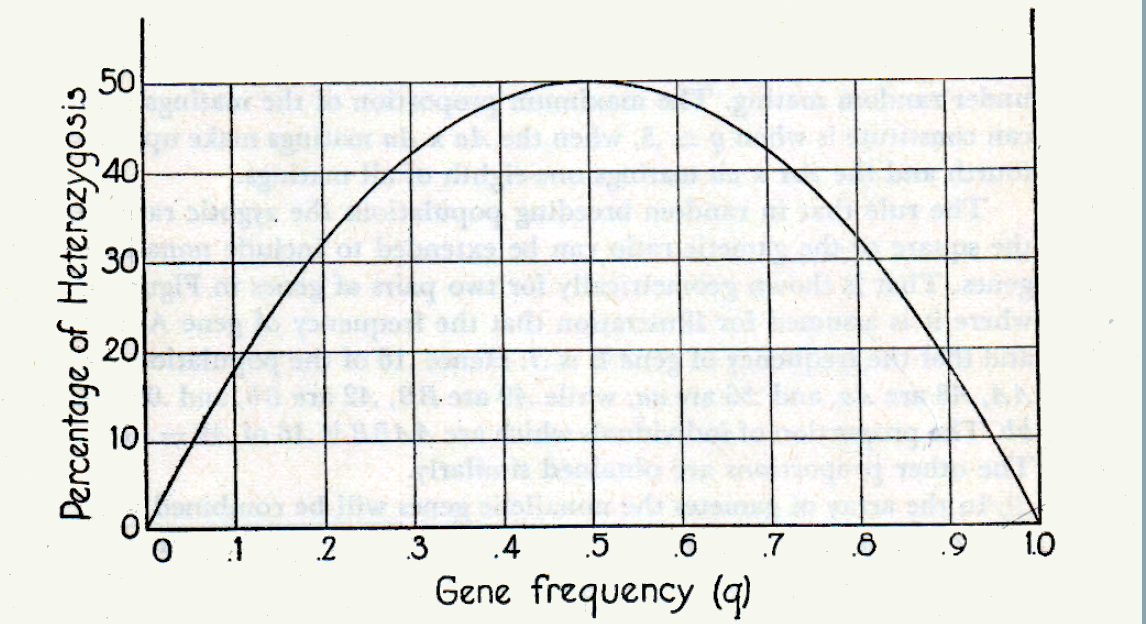
\includegraphics[width=\textwidth]{Figure_3.png}
    \caption{The percentage of heterozygosis as related to gene frequency in a random breeding population.}
    \label{fig:Lush_Figure_3}
\end{figure}

The frequency with which each kind of mating occurs depends much on \textit{q}. Thus, if there are
$q^{2}AA$ males and $q^{2}AA$ females and mating is at random, the most probable proportion of
matings of the type $AA \times AA$ is $q^2 \times q^2$, or $q^4$. Extending this to the other
five types of matings possible, where there are only two alleles, gives the proportions
shown in Figure~\ref{fig:Lush_Figure_4}. Matings of the kinds $AA \times AA$ or $aa \times aa$ can constitute
anything from none to all of the matings in the population according to the value of \textit{q}.
Matings of the kinds $AA \times Aa$ and $AA \times aa$ can constitute from none to 42 per cent
of the matings. The maximum figure is reached for the $AA \times Aa$ mating when \textit{q} = .75
and for the Aa x aa mating when q = .25. Regardless of q, matings of the type $Aa \times Aa$ are
always just twice as frequent as matings of the type $AA \times aa$ under random mating. The maximum
proportion of the matings they can constitute is when \textit{q} = .5, when the $Aa \times Aa$
matings make up one-fourth and the $AA \times aa$ matings one-eighth of all matings.
\index{Heterozygosis|)}

\begin{figure}[htbp]
    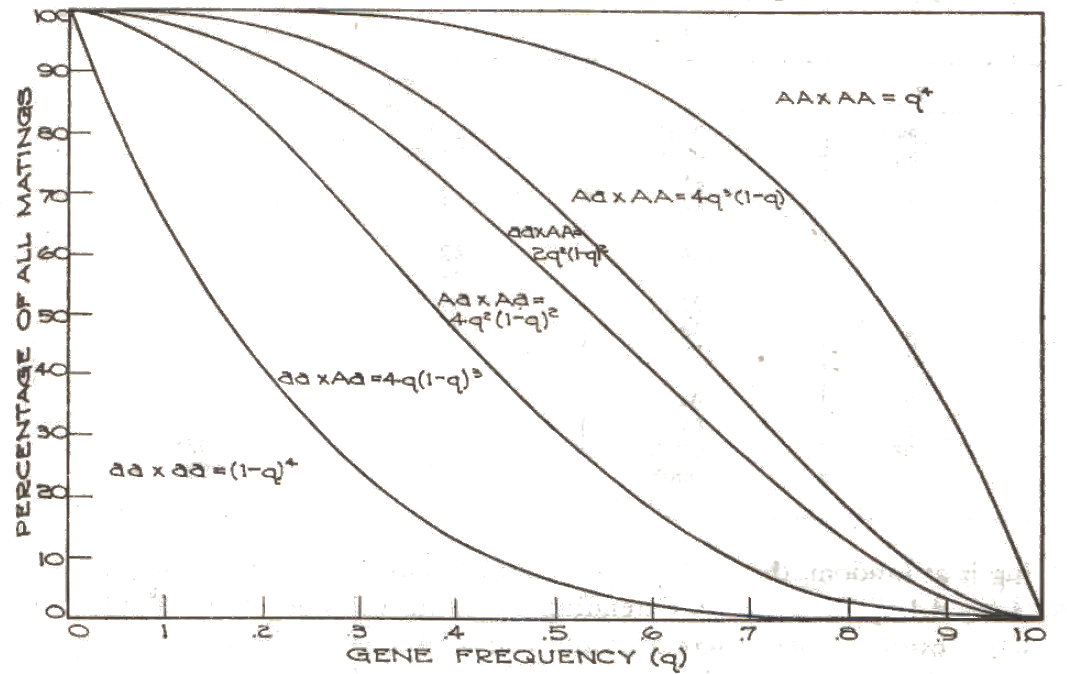
\includegraphics[width=\textwidth]{Figure_4.png}
    \caption[justification=justified]{Showing how the abundance or scarcity of each kind of mating changes with gene frequency in a population mating at random. Vertical distances are in proportion to the frequency of each
    		 kind of mating.}
    \label{fig:Lush_Figure_4}
\end{figure}

The rule that in random breeding populations the zygotic ratio is the square of the gametic ratio can be
extended to include nonallelic genes. That is shown geometrically for two pairs of genes in
Figure~\ref{fig:Lush_Figure_5}, where it is assumed for illustration that the frequency of gene A is .4
and that the frequency of gene B is .7. Hence .16 of the population are \textit{AA}, .48 are \textit{Aa},
and .36 are \textit{aa}; while .49 are \textit{BB}, .42 are \textit{Bb}, and .09 are \textit{bb}. The
proportion of individuals which are \textit{AABB} is .16 of .49 =.0784. The other proportions are obtained
similarly.

\begin{figure}[htbp]
    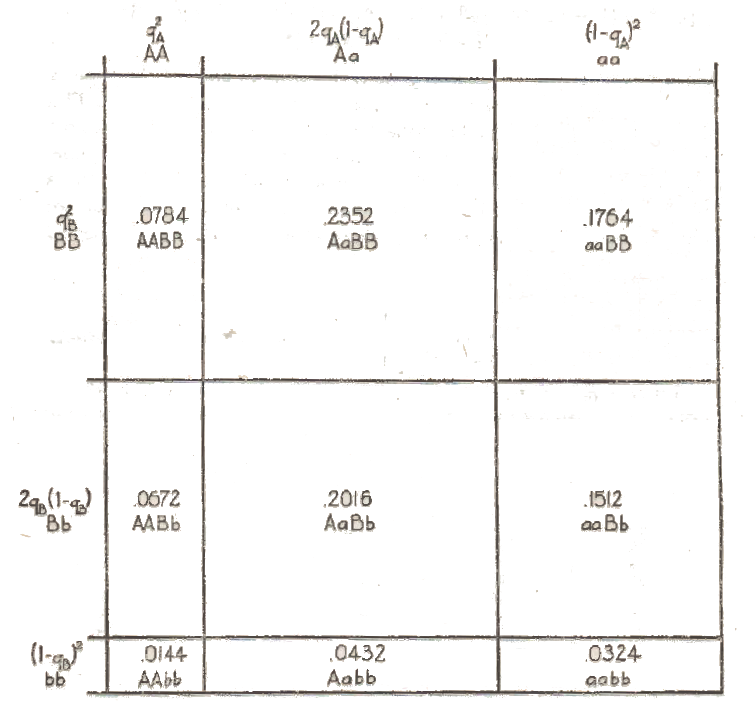
\includegraphics[width=\textwidth]{Figure_5.png}
    \caption{Showing how the rarity or abundance of the various genotypes in a random breeding population
    	     depends on the frequency of the genes in each pair.}
    \label{fig:Lush_Figure_5}
\end{figure}

In the array of gametes the nonallelic genes will be combined with each other independently except under
three circumstances. First, if the population is the result of a recent cross, the
\index{Coupling and repulsion}coupling and the
repulsion phases of linked genes may not yet have had time to become equally abundant. Second, if the
parents were produced by assortive mating (See Chapter 27), genes which produce similar
effects will be together in the same gametes more frequently than otherwise. Third, if the parents are a
selected group (rather than a random sample or a typical sample of their generation), the gametes they
produce will contain slightly fewer extreme combinations and more intermediate combinations than if the
same genes were combined entirely at random.

The two-factor $F_2$ ratio, used in genetics texts to introduce the subject of inheritance where more than
one pair of genes is involved, is only the special case in which the frequency of both genes is exactly .5.
The zygotic ratio when \textit{n} genes combine at random can be had by multiplying all the zygotic ratios
for each pair of genes together thus:

\begin{gather*}
	\left[ q_{A}A + (1-q_{A}a) \right]^2 + \left[ q_{B}B + (1-q_{B}b) \right]^2 +
	\left[ q_{C}C + (1-q_{C}c) \right]^2 + \ldots + \\ \left[ q_{N}N +
	(1-q_{N}n) \right]^2
\end{gather*}

\index{Homozygosis|(}
If the frequency of the desired gene is the same in each of the \textit{n} pairs,
the formula can be written in a simpler form: $[q_A + (1 - q_A)]^{2n}$. This
shows why the search for breeding animals homozygous in all desired genes has no
prospect for immediate success unless the number of genes desired is very small
and the desired gene in each pair already has a high frequency. Table~\ref{tbl:Lush_Table_3}
shows the expectation for various values of \textit{q} and \textit{n}, figures being shown
only where at least 1 in 1,000 is expected to exist.

\begin{center}
	\begin{table}[htbp]
		\caption{\textsc{Portion of Random Bred Population Which Will Be Homozygous For}
		\textit{n} \textsc{Desired Genes =} $q^{2}_{A}q^{2}_{B}q^{2}_{C} \ldots q^{2}_{N}$\\
		Let $q_A = q_B = q_C = \ldots = q_N$. Then portion equals $q^{2n}$}
		\label{tbl:Lush_Table_3}
		\begin{tabular}{C{2cm}|C{2cm}|C{2cm}|C{2cm}|C{2cm}}
			\hline
			\hline
						& \multicolumn{4}{c}{\textit{n}} \\
			\cline{2-5}
			\textit{q}	& 5		& 10		& 20		& 50 \\
 			\hline
			.50			& .001	& \ldots	& \ldots	& \ldots \\
			.60			& .006	& \ldots	& \ldots	& \ldots \\
			.70			& .028	& .001		& \ldots	& \ldots \\
			.80			& .107	& .012		& \ldots	& \ldots \\
			.90			& .349	& .122		& .015		& \ldots \\
			.95			& .599	& .358		& .128		& .006 \\
			.98			& .817	& .668		& .446		& .133 \\
			.99			& .904	& .818		& .669		& .366 \\
 			\hline
		\end{tabular}
	\end{table}
\end{center}

Animals having at least one desirable gene in each pair but not
necessarily homozygous for all those pairs are much more frequent.
Thus, if $q^2$ are \textit{AA} and $2q(1 - q)$ are \textit{Aa}, those
which carry \textit{A} either in the homozygous or in the heterozygous
condition are $q^2 + 2q(l - q)$, which may be written $q(2 - q)$.
Extending this to \textit{n} pairs of genes gives the figures shown in
Table~\ref{tbl:Lush_Table_4}. Animals possessing at least one desired
gene in each pair are more apt to exist in large enough proportions that
it will be finitely possible to find them and to breed from them, discarding
all which do not come up to this standard, than is the case with
animals homozygous for the desired genes.

\begin{table}[htbp]
	\centering
	\caption{\textsc{Portion of Random Bred Population Which Will Possess at Least One
	Desired Gene in Each Pair =} $q_A(2-q_A)q_B(2-q_B)q_C(2-q_C) \ldots q_N(2-q_N)$.\\
	If $q_A = q_B = q_C = \ldots = q_N$, then portion equals $[q{2-q}]^n$}
	\label{tbl:Lush_Table_4}
	\begin{tabular}{C{2cm}|C{2cm}|C{2cm}|C{2cm}|C{2cm}}
		\hline
		\hline
					& \multicolumn{4}{c}{\textit{n}} \\
		\cline{2-5}
		\textit{q}	& 5			& 10		& 20		& 50 \\
 		\hline
		.30			& .035		& .001		& \ldots	& \ldots \\
		.50			& .237		& .056		& .003		& \ldots \\
		.70			& .624		& .389		& .152		& .009 \\
		.80			& .815		& .665		& .442		& .130 \\
		.90			& .951		& .904		& .818		& .605 \\
		.95			& .988		& .975		& .951		& .882 \\
		.99			& .999		& .999		& .998		& .995 \\
 		\hline
	\end{tabular}
\end{table}

In any actual population some of the animals will come nearer than
others to having all the desired genes, even though none of them perhaps
comes close to that ideal. The practical breeder's simplest reasonable
hope is that by selection he can steadily increase the frequency of
the desirable genes until sometime --- perhaps not until after many
generations --- they may reach such a high frequency that perfect breeding
animals may be born in his herd. But whether or not that goal is actually
attained in his lifetime, the increasing frequency of the desired genes
will carry the average merit of the population with it, so that he can
reap the reward for his efforts in each generation in which there actually
is any increase in the frequency of the desirable genes.

In most circumstances the practical breeder is much more interested
in average genetic merit than in homozygosity itself. For example, if
10 pairs of genes affect a trait and a breeder is choosing between one
animal which is homozygous for five of the desired genes but homozygous
for the undesired gene in the other five pairs and another animal
which is \index{Heterozygosis}heterozygous for all 10 pairs, there will be little difference in
their breeding usefulness to him. Each has 10 desired genes. On the
average each will transmit five desired genes to an offspring, the former
to every offspring without exception and the latter sometimes more and
sometimes less than five. Probably the wiser choice would be for the
more heterozygous animal since the greater variability of its offspring
offers more chance for rapid progress by selection among them.
\index{Gametic ratio|)}
\index{Gene frequency|)}
\index{Homozygosis|)}

\section*{DEVIATIONS FROM RANDOM MATING AS THEY AFFECT THE BINOMIAL DISTRIBUTION OF ZYGOTES}

Mating is random when mates are no more and no less like each
other than if they were paired by drawing numbers out of a hat. Random
mating does not mean promiscuity or carelessness. Deviations
from random mating may be of four genetically different kinds: (1)
inbreeding, (2) outbreeding, (3) mating like to like on the basis of
somatic resemblance, and (4) mating individuals which are somatically
unlike each other. There can, of course, be breeding systems which
involve combinations or alternations of two or more of these. Selection,
which is deciding that certain individuals shall have many offspring
while others shall have few or none, may be practiced along with
random mating among those selected to be parents. An illustration is
the breeding practiced on large ranches where sires and dams may be
highly selected to conform to the owner's standards, but after the selections
are made, several sires and many females are turned loose in the
same pasture and the matings within that pasture are random, so far as
concerns any human control over them. This is selection plus random
mating within the group selected to be parents. If the ideals toward
which the selections are made differ on different ranches, mating may
be random within the limits of each ranch but will not be random with
respect to the whole breed, since animals of like types will tend to be on
the same ranch and therefore will mate together more often than would
be the case if all the sires and dams on all the ranches were in one pasture.

Each of these systems of breeding which is not random will be the
subject of a later chapter. Inbreeding tends to make the array of zygotes
more like that which would exist if the array of gametes were changed
into zygotes by doubling all the genes in each gamete. Inbreeding promotes
the formation of families of all kinds, thus adding to the diversity
of the population. Outbreeding, which prevails when mates are less
closely related to each other than if they were mating at random, is the
reverse of inbreeding and cancels many of its effects. It is especially
potent in destroying family differences which have been produced hy
inbreeding, and at producing hybrid vigor or \index{Heterosis}``heterosis.'' Unless distinct
families already exist, outbreeding cannot be carried far. The
general effect of mating like to like, within the whole group of parents
selected to produce the next generation of the breed, is to make the
population more variable by providing more than a random chance for
gametes from an extreme individual to meet with gametes from an individual
which is extreme in the same direction. The mating of unlikes
together makes the population more uniform by making it more likely
that gametes from an extreme individual will unite with gametes from
an individual extreme in the opposite direction than would be the
case under strictly random mating. It is the most potent breeding system
for producing immediate uniformity in a population but produces
nearly all its effects in the first generation practiced. It is practiced
much where the ideal is intermediate and the breeder seeks to mate
them so that each will compensate for the defects of its mate.
\index{Binomial distribution|)}
\index{Random mating|)}
\index{Zygotic ratios|)}

\section*{REFERENCES}

\begin{hangparas}{0.5in}{1}%
Belling, John. 1931. Chromomeres of liliaceous plants. Univ. Calif. Pub. Bot., 16:
153--70.

Cole, L. J., and Jones, Sarah V. H. 1920. The occurrence of red calves in black
breeds of cattle. Wisconsin Agr. Exp. Sta., Bul. 313.

Fisher, R. A. 1930. The genetical theory of natural selection. (See especially pp.
17--18 and 38--41.)

Gowen, John W., and Gay, E. H. 1933. Gene number, kind, and size in Drosophila.
Genetics, 18:1--31.

Ibsen, H. L. 1933. Cattle inheritance. I. Color. Genetics, 18:441--80.

Juli, M. A. 1934. The inheritance of sexual maturity, rate, and persistency of laying
in the domestic fowl. Poultry Science, 13:286--89.

King, H. D. 1932. Mutations in a strain of captive gray Norway rats. Proc. Sixth
Internat. Cong. of Genetics, 2:108--10.

Muller, H. J., and Prokofyeva, A. A. 1935. The individual gene in relation to the
chromomere and the chromosome. Proc. Nat. Acad. Sci., 21: 16--26.

Rhoades, M. M., and McClinLock, Barbara. 1935. The cytogenetics of maize. Botanical
Review, 1:292--325.

Skovsted, A. 1932. Nordisk Jordbrugsforskning, 5:201--5.

Stadler, L. J. 1932. On the genetic nature of induced mutations in plants. Proc.
Sixth Internat. Cong. of Genetics, 1:274--94.

``Student.'' 1934. A calculation of the minimum number of genes in Winter's
selection experiment. Annals of Eugenics, 6(Part 1):77--82.

Sumner, F. B. 1932. Genetic distributional and evolutionary studies of the subspecies
of deer-mice (Peromyscus). Bibliographia Genetica, 9:1-106.

Wriedt, Chr. 1929. Den mendelske spaltning av fettprosenten ved kryssning av r{\o}dt
dansk og jerseyfe. Nordisk Jordbrugsforskning, 103--21.
\end{hangparas}